\documentclass[10pt,letterpaper]{article}

\usepackage[margin=1in]{geometry}
\usepackage{iftex}
% mathptmx has no TU-encoded faces, so under XeTeX (Tectonic) earlier versions fell back
% to Latin Modern regular and lost every bold and italic. Use Termes there.
\ifPDFTeX\usepackage{mathptmx}\else\usepackage{fontspec}\setmainfont{texgyretermes}[Extension=.otf,UprightFont=*-regular,BoldFont=*-bold,ItalicFont=*-italic,BoldItalicFont=*-bolditalic]\fi
\usepackage{textcomp}
\usepackage{amsmath}
\usepackage{graphicx}
\usepackage{booktabs}
\usepackage{listings}
\usepackage{xcolor}
\usepackage{tikz}
\usetikzlibrary{positioning,arrows.meta,fit,backgrounds,calc}
\usepackage{natbib}
\usepackage[colorlinks=true,linkcolor=blue,citecolor=blue,urlcolor=blue]{hyperref}
\usepackage{microtype}
\usepackage{parskip}
\usepackage{titlesec}
\usepackage{enumitem}
\usepackage{caption}

\setlength{\parskip}{6pt}
\setlength{\parindent}{0pt}
\setlength{\emergencystretch}{3em}

\lstset{
  basicstyle=\small\ttfamily,
  breaklines=true,
  frame=single,
  numbers=left,
  numberstyle=\tiny,
  xleftmargin=2em,
  framexleftmargin=1.5em,
  backgroundcolor=\color{gray!8},
}

\definecolor{claimcolor}{RGB}{0,70,140}
\newcounter{claim}
\newenvironment{property}[1][]{%
  \refstepcounter{claim}%
  \vspace{4pt}%
  \noindent\fbox{\parbox{\dimexpr\linewidth-2\fboxsep-2\fboxrule}{%
    \textbf{\textcolor{claimcolor}{Property \theclaim} (#1).}
}}\par\vspace{2pt}%
}{\vspace{4pt}}

\title{\textbf{cMCP: Verifiable Policy Enforcement for AI Agent Tool Calls}}

\author{
  Rishabh Poddar \quad Aaron Fulkerson \quad Imran Siddique \\
  OPAQUE Systems \\[4pt]
  \normalsize \url{https://github.com/agentrust-io/cmcp}
}

\date{October 1, 2026 \\ \small Technical report, version 2}

\begin{document}

\maketitle

\begin{abstract}
cMCP (Confidential MCP) proposes a gateway for policy evaluation at the
Model Context Protocol tool-call boundary. The gateway evaluates Cedar policies
before dispatch and emits signed records binding policy measurements, session
identifiers, and tool-call evidence. Its design combines policy hashing,
monotonic session sensitivity, tool-catalog pinning, and audit-chain checks.
This technical report preserves software-only experiments for those mechanisms,
including synthetic healthcare call traces and simulated attestation paths.
The measurements illustrate behavior under the stated inputs and assumptions;
they do not validate a hardware TEE, establish complete information-flow tracking,
or show that every tool invocation was captured. Hardware provenance requires
independent attestation appraisal and signing-key binding. Replay and omission
detection additionally depend on freshness checks and an expected session or log
boundary. The report distinguishes these deployment requirements from the
software behavior measured here.
\end{abstract}

\paragraph{Scope of this edition.}
This is an author-prepared technical report, not peer reviewed and not a
normative specification. Version 2 corrects version 1 (September 27, 2026) where the
text did not match the code or the experiments: the size of the hardware
\texttt{REPORT\_DATA} field, the nonce the session claim carries, when the catalog check
runs, trial counts the experiments do not perform, two misattributed citations, and two
misread performance figures. It restores bold and italic type that the Tectonic build had dropped, and names the measured revision and the published
security advisories that affect it. Every experiment was rerun on October 1, 2026 against
cMCP commit \texttt{6f12cce} (\texttt{cmcp-runtime} 0.3.0 plus four commits, the
repository state when the performance numbers were recorded); correctness results are
unchanged. Version 1 revised a manuscript dated June 23, 2026. Architectural requirements describe intended checks, not proof that
the historical SDK implements every check. Consult the linked project
specification and limitations before implementing the design.

\noindent\textbf{Patent Pending.}

\tableofcontents
\newpage

\section{Introduction}
\label{sec:intro}

AI agents that use tools are rapidly becoming the dominant pattern for deploying language
models in production. A single user request may cause an agent to invoke a dozen tools:
reading email, querying a database, calling an external API, posting to a messaging system.
Each tool call crosses a trust boundary. The tool may be provided by a third party, run on
a different server, or handle regulated data. Yet the agent's orchestration layer has no
standard mechanism for verifying what policies governed the call, who authorized the
invocation, or whether the returned data places compliance obligations on everything the
agent does next.

Model Context Protocol (MCP)~\citep{mcp2024} formalizes this interaction as a JSON-RPC
protocol with standardized tool discovery and invocation semantics. MCP has seen rapid
adoption: within a year of publication, hundreds of MCP servers expose tools ranging from
filesystem access to medical record retrieval. This adoption makes the governance gap concrete.
When an agent calls \texttt{ehr.get\_patient} through an MCP server and the response contains
protected health information, nothing in the MCP protocol tells the agent, its orchestrator,
or a downstream auditor: which policy authorized this call; whether the response sensitivity
has been tracked; whether the tool definition matches what was reviewed at deployment time.

cMCP addresses this gap. It is a TEE-based gateway that sits between an MCP client and one or
more MCP servers. Every tool call passes through cMCP, which evaluates Cedar~\citep{cedar2023}
policies before dispatch and, after the call completes, appends a signed entry to a
hash-chained audit log. At session close, cMCP produces a TRACE Claim~\citep{trace2025}: a
cryptographically signed attestation that binds the session's call record to the TEE instance
that processed it and to the policy bundle in effect at startup.

The central thesis of this paper is that hardware attestation, applied at the MCP boundary,
can provide verifiable governance properties that cannot be achieved through software-only
interception. We validate six such properties through reproducible experiments, each backed by
unit tests that run in CI without hardware TEE; the experiments establish the
software-checkable behavior of each property, while the binding to physical hardware is
architectural and is stated as a limitation (Section~\ref{sec:eval}).

\subsection*{Contributions}

\begin{itemize}[leftmargin=1.5em]
  \item \textbf{cMCP architecture.} A TEE gateway design that is transparent to existing MCP
    clients and servers, requiring no protocol changes.

  \item \textbf{TEE-measured policy enforcement (Property~\ref{prop:policy-hash}).} Policy
    bundles are measured into the TEE at startup. Any runtime modification raises
    \texttt{PolicyHashMismatch} and invalidates the TRACE Claim signature.

  \item \textbf{Session sensitivity tracking (Property~\ref{prop:session-sensitivity}).}
    A monotonically increasing session sensitivity state machine detects PHI cross-boundary
    violations that per-call policy evaluation cannot see, at a quantified false-discovery cost.

  \item \textbf{Rug-pull detection (Property~\ref{prop:rug-pull}).} Tool catalog entries are
    hash-pinned at TEE startup. Any post-approval modification to a tool's description or
    input schema triggers fail-closed rejection before the call is dispatched.

  \item \textbf{TRACE Claim key binding (Property~\ref{prop:nonce}).} Each TRACE Claim
    carries a nonce formed from the RFC~7638 JWK Thumbprint of the TEE public key and a
    random salt, committed into the hardware report; the per-session report replaces the
    salt with a hash of the session's audit-chain root. A verifier re-derives the
    thumbprint from the claim's confirmation key to bind the report to the signing key, and
    the session identifier is covered by the claim signature. Detecting replay and omission
    additionally needs a freshness check and an expected session boundary.

  \item \textbf{Temporal adjacency provenance (Property~\ref{prop:temporal}).} cMCP
    records a call graph where edges represent temporal adjacency. This is a conservative
    provenance approximation: zero false negatives by construction, with a quantified false
    positive rate.

  \item \textbf{Cross-organizational attestation chains (Property~\ref{prop:cross-org}).}
    A dual-TEE protocol links independent Phase~1 (gateway) and Phase~2 (server) TRACE
    Claims through a shared session identifier and independently verifiable nonces.
\end{itemize}

\subsection*{Paper structure}

Section~\ref{sec:background} covers MCP mechanics, TEE attestation, the TRACE standard,
Cedar policies, and the threat model. Section~\ref{sec:design} describes the cMCP
architecture and its key mechanisms. Section~\ref{sec:claims} formally states the six
security properties. Section~\ref{sec:eval} presents experimental validation of each
property with quantitative results. Section~\ref{sec:related} surveys related work.
Section~\ref{sec:conclusion} concludes.

\section{Background}
\label{sec:background}

\subsection{Model Context Protocol}

Model Context Protocol (MCP)~\citep{mcp2024} is a JSON-RPC~2.0 protocol that standardizes
how AI agents discover and invoke tools hosted on external servers. A \emph{tool} is a named
function with a JSON Schema describing its parameters. MCP defines three primitive operations:
\texttt{tools/list} to enumerate available tools, \texttt{tools/call} to invoke one, and
\texttt{resources/read} to retrieve structured data.

An MCP session begins when a client establishes a transport connection (Streamable HTTP,
which replaced HTTP with Server-Sent Events in the 2025-03-26 revision, or stdio) to an MCP
server and exchanges \texttt{initialize} messages.
The server advertises its tool catalog; the client may cache it. Subsequent tool calls are
stateless from the protocol's perspective: each \texttt{tools/call} carries the tool name
and a JSON argument object and receives a JSON content array in response.

MCP's authorization specification, added in the 2025-03-26 revision, uses OAuth 2.1 to
authorize a client's access to a server. It does not define a per-call policy decision over
tool arguments or session history, does not require any audit record of calls made, and
does not provide a mechanism for a client to verify that the tool definition it cached at
session start is still the definition the server will execute. These gaps are the governance problem
cMCP addresses.

\subsection{Trusted Execution Environments}

A Trusted Execution Environment (TEE) is a CPU-enforced isolation boundary that provides
two guarantees relevant to this paper: \emph{confidentiality} (memory within the TEE is
inaccessible to software outside, including the hypervisor and OS) and
\emph{remote attestation} (the TEE can produce a hardware-signed measurement report that
proves, to a remote verifier, which code is running inside).

The measurement report is the key primitive. On AMD SEV-SNP~\citep{amdsevsnp2023}, the
report is signed by the AMD attestation key (VCEK) and includes a 64-byte
\texttt{REPORT\_DATA} field that the guest can set to arbitrary bytes. On Intel
TDX~\citep{inteltdx2023}, the equivalent field is the 64-byte \texttt{REPORTDATA}. cMCP uses this field to bind application-level
context (specifically, the session nonce) to the hardware attestation, as described in
Section~\ref{sec:design}.

In software-only mode, cMCP substitutes a software-generated key and produces a synthetic
attestation report marked with \texttt{platform: software-only}. Software-only TRACE Claims
carry \texttt{attestation\_assurance: none} and must not be used for compliance decisions.
All experiments in this paper run in software-only mode.

\subsection{TRACE Standard}

TRACE (Trust Runtime Attestation and Compliance Evidence)~\citep{trace2025} is an open
attestation standard for agentic AI. A TRACE Claim is a JSON document with two top-level
sections: a canonical \emph{trace} envelope (eat\_profile, issued-at timestamp, subject
identifier, runtime measurement, policy reference, data classification, confirmation key)
and a profile-specific addenda section that carries deployment context.

The cMCP profile of TRACE adds a \emph{gateway addenda} section containing: the session
identifier, gateway version, a monotonically increasing sequence number for claim ordering,
an audit chain summary (root hash, tip hash, chain length), a call summary (total calls,
allowed, denied, faulted, tools invoked, maximum session sensitivity), a catalog hash, and
attestation freshness fields. The claim is signed with an Ed25519 key whose public half
appears in the \texttt{cnf} (confirmation key) field, allowing any verifier to check the
signature without contacting the gateway.

\subsection{Cedar Policy Language}

Cedar~\citep{cedar2023} is a policy language and evaluation engine developed by AWS. Cedar
policies express access control decisions as \texttt{permit} or \texttt{forbid} rules over
a triple of \emph{principal} (who is making the request), \emph{action} (what is being
requested), and \emph{resource} (what is being acted on), with optional \texttt{when}
conditions evaluated against a context object.

cMCP evaluates Cedar policies at tool-call time. The principal is the agent's SPIFFE
identity~\citep{spiffe2018}, the action is the tool name, and the resource is the MCP server
URL. The context includes the tool's compliance domain (e.g., \texttt{phi}, \texttt{pii},
\texttt{confidential}), the current session sensitivity level, and the call's input
parameters. Cedar's structural typing ensures that policy evaluation is decidable in
bounded time, a property important for a gateway that must not add unbounded latency.

\subsection{Threat Model}

cMCP assumes the following attacker capabilities:

\textbf{T1: Policy modification.} An attacker with access to the gateway host can modify
the Cedar policy files after TEE startup, attempting to relax enforcement for subsequent
calls.

\textbf{T2: Tool catalog tampering.} An attacker can modify an MCP server's tool
definitions after the gateway has cached them, replacing a benign implementation with one
that exfiltrates data or behaves differently than the approved specification.

\textbf{T3: Claim replay.} An attacker intercepts a TRACE Claim produced for one session
and presents it as evidence for a different session, a different TEE instance, or a future
point in time.

\textbf{T4: Selective disclosure.} An attacker selectively presents audit entries from a
TRACE Claim, omitting evidence of non-compliant calls while presenting evidence of compliant
ones.

\textbf{T5: Cross-boundary data exfiltration.} An agent that has processed regulated data
(PHI, PII) subsequently calls external tools in a way that the orchestrator cannot detect,
because the PHI was in an intermediate agent state rather than in the tool call parameters.

\textbf{T6: Binary substitution.} In a cross-organizational setting, the server-side TEE
binary is swapped after the gateway has verified the server's attestation report, allowing
the new binary to behave differently without re-attestation.

cMCP does not address denial-of-service against the gateway itself, compromise of the CPU
manufacturer's signing key, or attacks that require the TEE's measurement to be forged. It
also does not address semantic attacks where a malicious tool produces a compliant-looking
response that causes the agent to take harmful downstream actions.

\section{cMCP Design}
\label{sec:design}

\subsection{Architecture Overview}

cMCP is a transparent MCP proxy. An MCP client connects to cMCP as if connecting to an MCP
server; cMCP connects to one or more upstream MCP servers as an MCP client. The client
requires no modification. Figure~\ref{fig:arch} sketches the component layout.

\begin{figure}[h]
\centering
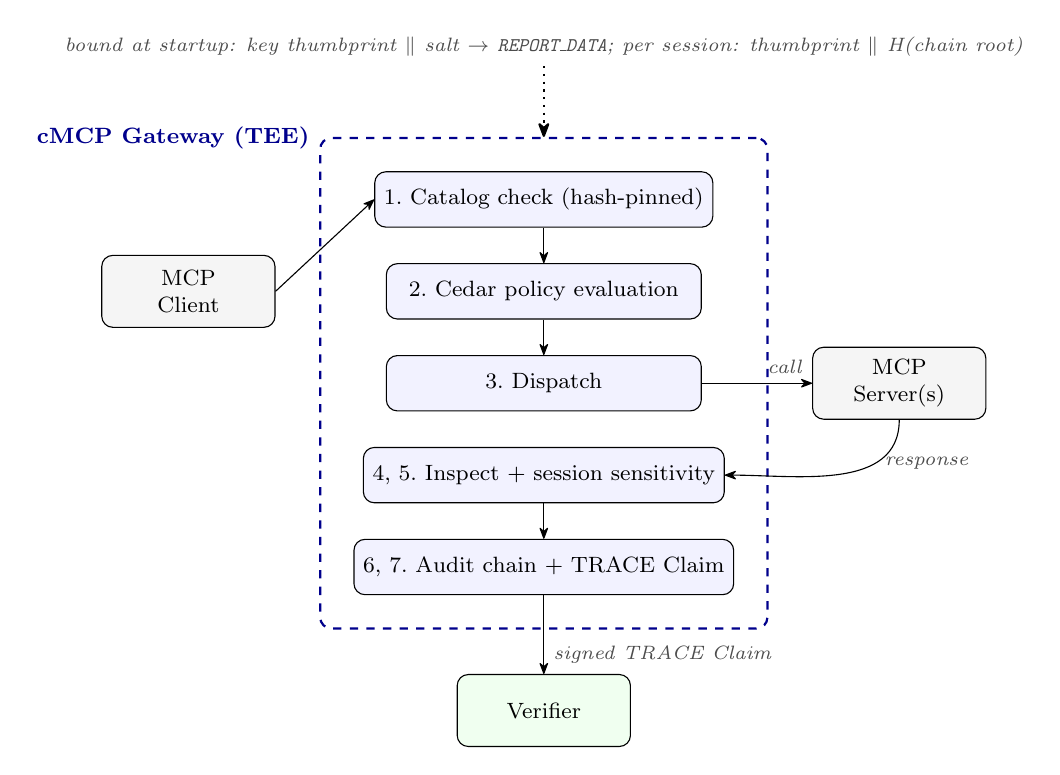
\begin{tikzpicture}[
  font=\footnotesize,
  >={Stealth[round]},
  endpoint/.style={draw, rounded corners, minimum width=2.2cm, minimum height=2.6em, align=center, fill=gray!8},
  stage/.style={draw, rounded corners, minimum width=4.0cm, minimum height=2.0em, align=center, fill=blue!5},
  tee/.style={draw, dashed, thick, rounded corners, draw=blue!55!black, inner sep=12pt},
  note/.style={align=center, font=\scriptsize\itshape, text=black!70},
]
% Gateway internal pipeline (vertical)
\node[stage] (catalog) {1.\ Catalog check (hash-pinned)};
\node[stage, below=0.45cm of catalog] (cedar) {2.\ Cedar policy evaluation};
\node[stage, below=0.45cm of cedar] (dispatch) {3.\ Dispatch};
\node[stage, below=0.45cm of dispatch] (inspect) {4, 5.\ Inspect + session sensitivity};
\node[stage, below=0.45cm of inspect] (audit) {6, 7.\ Audit chain + TRACE Claim};

% TEE boundary
\begin{scope}[on background layer]
  \node[tee, fit=(catalog)(cedar)(dispatch)(inspect)(audit),
        label={[text=blue!55!black]above left:\textbf{cMCP Gateway (TEE)}}] (gw) {};
\end{scope}

% External endpoints
\node[endpoint, left=1.4cm of cedar] (client) {MCP\\Client};
\node[endpoint, right=1.4cm of dispatch] (server) {MCP\\Server(s)};
\node[endpoint, below=1.0cm of audit, fill=green!6] (verifier) {Verifier};

% Request / response flow
\draw[->] (client.east) -- (catalog.west);
\draw[->] (catalog) -- (cedar);
\draw[->] (cedar) -- (dispatch);
\draw[->] (dispatch.east) -- node[note, above, pos=0.75]{call} (server.west);
\draw[->] (server.south) to[out=270,in=0] node[note, right, pos=0.3]{response} (inspect.east);
\draw[->] (inspect) -- (audit);

% Startup measurement and output
\node[note, above=0.9cm of gw.north] (meas)
  {bound at startup: key thumbprint $\|$ salt $\rightarrow$ \texttt{REPORT\_DATA}; per session: thumbprint $\|$ H(chain root)};
\draw[->, dotted, thick] (meas) -- (gw.north);
\draw[->] (audit.south) -- node[note, right, pos=0.75]{signed TRACE Claim} (verifier.north);
\end{tikzpicture}
\caption{cMCP interposes on every tool call between an MCP client and upstream MCP
servers. The numbered stages correspond to the tool-call flow in
Section~\ref{sec:design}. The gateway key is bound into the attestation report at startup,
and each session's report also commits the audit-chain root; policy-bundle and catalog
hashes travel in the signed TRACE Claim, which lets an external verifier confirm what
governed the session.}
\label{fig:arch}
\end{figure}

At startup, cMCP performs four initialization steps before accepting any connections: (1) it
generates a fresh Ed25519 keypair whose private half never leaves TEE memory; (2) it loads
the Cedar policy bundle, records its SHA-256 hash, and refuses to start if the hash differs
from a configured expected value; (3) it loads the operator-approved tool catalog file,
records the aggregate catalog hash, and applies the same expected-hash check; and (4) it
obtains an attestation report from the TEE with \texttt{REPORT\_DATA} set to the key
nonce described below. The policy and catalog hashes are carried in
the signed claim body rather than in \texttt{REPORT\_DATA} at the measured revision.

\subsection{Tool Call Flow}

When the MCP client sends a \texttt{tools/call} request, cMCP executes the following
sequence:

\begin{enumerate}[leftmargin=1.5em]
  \item \textbf{Catalog check.} Verify that the requested tool is in the pinned catalog and
    that the in-memory catalog hash still equals the startup hash. If it does not, the
    session is marked \texttt{catalog\_drift} and the call is refused.
  \item \textbf{Cedar evaluation.} Evaluate the Cedar policy bundle against the call
    context. If the decision is \texttt{forbid}, return a policy-denial response immediately
    without forwarding the call.
  \item \textbf{Dispatch.} Forward the call to the upstream MCP server.
  \item \textbf{Inspection.} Pass the response through the \texttt{InspectionPipeline},
    which classifies sensitivity tags (e.g., \texttt{hipaa\_phi}, \texttt{pii}) and detects
    prompt-injection patterns.
  \item \textbf{Session state update.} Call \texttt{update\_from\_inspection()} on the
    session's \texttt{SessionState}, which may raise the session sensitivity level.
  \item \textbf{Audit append.} Append a hash-chained entry to the session's audit log,
    recording the tool name, policy decision, sensitivity tags, and the previous entry's
    hash.
  \item \textbf{Call log record.} Record the call in the session's \texttt{SessionCallLog}
    with a monotonically increasing sequence number, for temporal adjacency tracking.
\end{enumerate}

Steps 1 and 2 must both pass for the call to proceed. A Cedar allow decision does not
bypass the catalog check, and a clean catalog does not bypass Cedar.

\subsection{Session Sensitivity State Machine}

Each session maintains a \texttt{SessionState} object with a \texttt{max\_sensitivity}
field. The sensitivity order is:

\[
  \text{public}(0) < \text{pii}(1) < \text{confidential}(2) < \text{hipaa\_phi} = \text{mnpi} = \text{trade\_secret}(3)
\]

\texttt{max\_sensitivity} is initialized to \texttt{public} and transitions only upward:
whenever the inspection pipeline tags a response with a higher sensitivity level, the state
machine raises \texttt{max\_sensitivity} to that level and records which call triggered the
transition. The session sensitivity never decreases automatically. An operator reset, which
rotates the session identifier, is the only way to lower it.

This monotonic design is the source of both its guarantee and its cost. It guarantees that
once PHI enters the session context, every subsequent external call is attributed as
potentially PHI-adjacent. It causes false positives when a subsequent external call is
provably unrelated to the PHI. Calls can now declare a sensitivity class through
\texttt{\_cmcp.data\_class}, but the declaration is agent-cooperative input rather than an
independently proven lineage fact.

\subsection{Tool Catalog Pinning}

At startup, cMCP computes a definition hash for each tool:

\[
  h_{\text{tool}} = \text{SHA-256}(\text{tool\_name} \| \text{description} \| \text{inputSchema})
\]

where the fields are serialized as canonical JSON with sorted keys. The aggregate catalog
hash is SHA-256 of the sorted concatenation of all per-tool hashes. Both hashes are stored
in TEE-protected memory.

The approved catalog is an operator-curated file, not a live fetch. A catalog whose hash
differs from the expected value raises \texttt{CatalogHashMismatch} at load time and the
gateway does not start. Clients receive \texttt{tools/list} from the approved catalog, so a
description an upstream server changes after approval never reaches the agent. Before every
\texttt{tools/call}, the gateway compares the in-memory catalog hash with the startup value
and refuses the call on a mismatch. At the measured revision it does not compare the
upstream server's own \texttt{tools/list} with the approved entry; that comparison was added
later (Section~\ref{sec:eval}, Limitations). Hashing a definition cannot detect a server
that keeps its advertised definition and changes its behavior.

\subsection{TRACE Claim Generation}

At session close (or on demand), cMCP produces a TRACE Claim by:

\begin{enumerate}[leftmargin=1.5em]
  \item Computing the session nonce:
    $\text{nonce} = \text{TP}(\text{pubkey}) \,\|\, \text{SHA-256}(\text{chain\_root})$, the
    32-byte RFC~7638 JWK Thumbprint of the gateway public key followed by the hash of the
    session's first audit entry, which records the session identifier. The startup report
    uses a 32-byte random salt in place of the chain-root hash.
  \item Requesting an attestation report from the TEE with \texttt{REPORT\_DATA} set to the
    64-byte nonce (which fills the field exactly). This happens when the session opens; if
    the call fails, the claim falls back to the startup report and the verifier reports the
    chain-root binding as missing.
  \item Assembling the \texttt{RuntimeClaim} Pydantic model with the attestation report,
    policy bundle hash, catalog hash, session call summary, and audit chain tip.
  \item Signing the canonical JSON serialization (sorted keys, no whitespace) of the claim
    body with the TEE's Ed25519 private key.
  \item Embedding the signature as a base64url-encoded field in the claim.
\end{enumerate}

The nonce construction binds the attestation report to the TEE instance: the first 32
bytes are the RFC~7638 JWK Thumbprint of the gateway public key, which a verifier
re-derives from the claim's \texttt{cnf.jwk} and compares to \texttt{REPORT\_DATA}$[{:}32]$,
confirming the report belongs to the key that signed the claim. The second half,
\texttt{REPORT\_DATA}$[32{:}64]$, commits the session's audit-chain root, so in hardware
mode the session is bound twice: by the hardware report and by the Ed25519 signature over
\texttt{session\_id}. Without the chain-root commitment an operator holding the signing
path could rebuild an internally consistent chain and re-sign it; this binding was added
in cMCP PR~\#368, before the measured revision.

\subsection{Cross-Organizational Attestation (Phase 2)}

When an MCP server also runs inside a TEE, the dual-TEE protocol extends the trust chain to
the server side (Figure~\ref{fig:dual-tee}). In Phase~2:

\begin{itemize}[leftmargin=1.5em]
  \item The server TEE generates its own Ed25519 keypair (Phase~2 key).
  \item At session start, both TEEs exchange public keys and agree on the shared session
    identifier.
  \item The Phase~2 nonce is the \emph{server} key thumbprint followed by its own salt,
    structurally identical to the Phase~1 nonce but bound to a different key. Both phases
    carry the shared session identifier in their signed claim bodies.
  \item The server TEE produces an independent TRACE Claim signed with the Phase~2 key.
\end{itemize}

\begin{figure}[h]
\centering
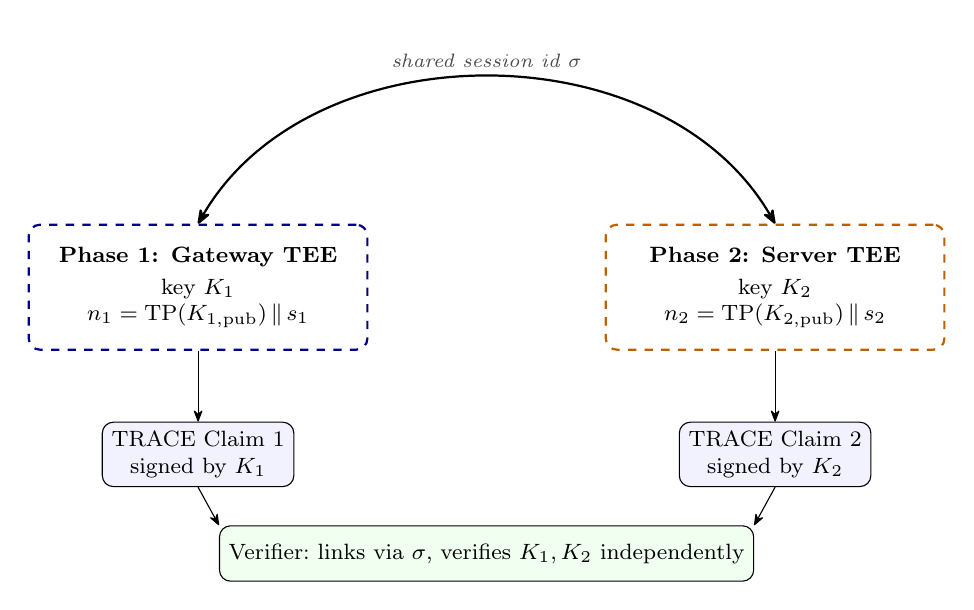
\begin{tikzpicture}[
  font=\footnotesize,
  >={Stealth[round]},
  tee/.style={draw, dashed, thick, rounded corners, align=center, minimum width=4.3cm,
              minimum height=4.2em, inner sep=8pt},
  claim/.style={draw, rounded corners, fill=blue!5, align=center, minimum height=2.0em},
  note/.style={font=\scriptsize\itshape, text=black!70},
]
\node[tee, draw=blue!55!black] (gw)
  {\textbf{Phase 1: Gateway TEE}\\[2pt] key $K_1$\\ $n_1=\text{TP}(K_{1,\text{pub}})\,\|\,s_1$};
\node[tee, draw=orange!75!black, right=3.0cm of gw] (srv)
  {\textbf{Phase 2: Server TEE}\\[2pt] key $K_2$\\ $n_2=\text{TP}(K_{2,\text{pub}})\,\|\,s_2$};

% shared session identifier link
\draw[<->, thick] (gw.north) to[out=60,in=120]
  node[note, above, pos=0.5]{shared session id $\sigma$} (srv.north);

\node[claim, below=0.9cm of gw] (c1) {TRACE Claim 1\\ signed by $K_1$};
\node[claim, below=0.9cm of srv] (c2) {TRACE Claim 2\\ signed by $K_2$};
\draw[->] (gw) -- (c1);
\draw[->] (srv) -- (c2);

\node[draw, rounded corners, fill=green!6, align=center, minimum height=2.0em,
      below=0.9cm of $(c1)!0.5!(c2)$] (ver) {Verifier:\ links via $\sigma$,\ verifies $K_1,K_2$ independently};
\draw[->] (c1.south) -- (ver.north west);
\draw[->] (c2.south) -- (ver.north east);
\end{tikzpicture}
\caption{The dual-TEE attestation chain (Property~\ref{prop:cross-org}). Two
independently generated TEE keys produce two TRACE Claims linked by a shared
session identifier $\sigma$ but verifiable independently: tampering with one
claim does not affect the other.}
\label{fig:dual-tee}
\end{figure}

A verifier who holds both claims can confirm: (a) both claims reference the same session
identifier; (b) the Phase~1 nonce is bound to the gateway TEE key; (c) the Phase~2 nonce
is bound to the server TEE key; (d) tampering with one claim does not affect the validity
of the other. The two claims are linked but independently verifiable.

Phase~2 server TEE deployment is in progress; the experiment in Section~\ref{sec:eval}
simulates the protocol in software.

\section{Security Properties}
\label{sec:claims}

We state six security properties of cMCP. Each property corresponds to a reproducible
experiment in Section~\ref{sec:eval}. The properties are stated as informal invariants
over the cMCP runtime; formal proofs are left for future work.

\begin{property}[TEE-Measured Policy Enforcement]
\label{prop:policy-hash}
Let $B$ be the Cedar policy bundle loaded at TEE startup, and let $h_B$ be its
SHA-256 hash recorded in TEE-protected memory. For any tool call processed after startup:
\begin{enumerate}[leftmargin=1.5em,label=(\alph*)]
  \item The gateway starts only if the hash of the loaded bundle equals the configured
    expected value; a bundle swapped on disk before startup raises
    \texttt{PolicyHashMismatch}. The measured revision does not re-hash the bundle in
    memory before each call.
  \item The TRACE Claim for the session carries $h_B$ in the \texttt{policy.bundle\_hash}
    field. A verifier who independently hashes the policy files can confirm they match.
  \item Altering the bundle hash in a signed TRACE Claim invalidates its Ed25519
    signature. A claim that the gateway itself signs over a different bundle verifies; it
    is caught by comparing its \texttt{policy.bundle\_hash} with the approved value.
\end{enumerate}
\end{property}

\begin{property}[Session Sensitivity Tracking]
\label{prop:session-sensitivity}
Let $S$ be a session, and let $T_{\text{phi}}$ be the first tool call in $S$ whose
response is tagged with a sensitivity level in
$\{\text{hipaa\_phi}, \text{mnpi}, \text{trade\_secret}\}$.
\begin{enumerate}[leftmargin=1.5em,label=(\alph*)]
  \item After $T_{\text{phi}}$, \texttt{max\_sensitivity} is raised to the highest tag
    observed and never decreases below that level for the remainder of $S$.
  \item Any subsequent Cedar evaluation in $S$ that uses the current session sensitivity as
    context will observe the raised level, allowing policies to enforce cross-boundary
    restrictions on all calls after $T_{\text{phi}}$.
  \item Per-call sensitivity evaluation (evaluating each call independently without session
    context) cannot enforce such restrictions, because the PHI sensitivity is in the session
    state, not in the parameters of the subsequent call.
\end{enumerate}
The operational cost of this guarantee is a nonzero false-discovery proportion: calls after
$T_{\text{phi}}$ that are provably unrelated to the PHI are nonetheless flagged.
We quantify this cost empirically in Section~\ref{sec:eval}.
\end{property}

\begin{property}[Tool Catalog Rug-Pull Detection]
\label{prop:rug-pull}
Let $C$ be the approved tool catalog loaded and hash-pinned at TEE startup. For any tool
call to tool $t$:
\begin{enumerate}[leftmargin=1.5em,label=(\alph*)]
  \item If $C$ still hashes to its startup value and $t$ is in $C$, the call proceeds to
    Cedar evaluation, and the agent only ever sees $t$'s approved definition.
  \item If $C$ differs from the approved hash at load, \texttt{CatalogHashMismatch} is
    raised and the gateway does not start. If the in-memory catalog changes after startup,
    the call is refused before dispatch and is not propagated to the upstream server.
  \item The per-tool hash function has the avalanche property: a single-character change
    in any field changes approximately half the bits of the output hash.
\end{enumerate}
\end{property}

\begin{property}[TRACE Claim Key Binding]
\label{prop:nonce}
Let $K$ be the TEE keypair generated at startup. The attestation nonce is
$n = \text{TP}(K_{\text{pub}}) \,\|\, s$, where $\text{TP}(K_{\text{pub}})$ is the
32-byte RFC~7638 JWK Thumbprint of the public key and $s$ is a 32-byte random salt
drawn once per enclave startup. The report a session claim carries uses
$s = \text{SHA-256}(\text{chain\_root})$ instead. The nonce is committed into the hardware
report's \texttt{report\_data} field. The session identifier $\sigma$ is also covered by
the Ed25519-signed claim body.
\begin{enumerate}[leftmargin=1.5em,label=(\alph*)]
  \item $\text{TP}(K_{\text{pub}})$ is deterministic and re-derivable by any verifier
    from the \texttt{cnf.jwk} public key, so the verifier confirms
    $\text{report\_data}[{:}32] = \text{TP}(K_{\text{pub}})$ (key binding).
  \item The salt $s$ makes nonces distinct across startups that share a key, with
    overwhelming probability. Freshness against a verifier's own challenge is not
    provided by $s$ and requires a verifier-supplied nonce.
  \item Distinct gateway instances produce distinct key thumbprints
    ($K_1 \neq K_2 \Rightarrow \text{TP}(K_{1,\text{pub}}) \neq \text{TP}(K_{2,\text{pub}})$
    with overwhelming probability), so a claim cannot be presented under a different
    TEE instance's identity.
  \item Session binding: $\sigma$ is covered by the Ed25519 signature over the claim body.
    Replacing $\sigma$ invalidates the signature, so a claim valid for session $\sigma_1$
    cannot be replayed as $\sigma_2$.
  \item Modifying any field of a TRACE Claim invalidates the Ed25519 signature computed
    over the canonical JSON serialization of the claim body.
  \item Removing audit entries from an exported, signed audit bundle changes its hash and
    invalidates the export signature. A verifier holding the claim can also recompute the
    chain tip from the entries it receives and compare it with the signed tip.
\end{enumerate}
\end{property}

\begin{property}[Temporal Adjacency Provenance Approximation]
\label{prop:temporal}
Let $L$ be the \texttt{SessionCallLog} for session $S$. Each entry $e_i \in L$ has a
monotonically increasing sequence number $\text{seq}(e_i)$.
\begin{enumerate}[leftmargin=1.5em,label=(\alph*)]
  \item Sequence numbers are strictly increasing: $i < j \Rightarrow \text{seq}(e_i) < \text{seq}(e_j)$.
  \item A cross-boundary event is recorded whenever a call to a tool in domain $D_2$ follows
    any call to a tool in a high-sensitivity domain $D_1 \in \{\text{phi}, \text{pii},
    \text{pci}, \text{restricted}\}$, and $D_2 \neq D_1$. (Current releases add
    \texttt{hipaa\_phi}, \texttt{mnpi} and \texttt{pci\_data} to this set.)
  \item Every call graph summary includes a \texttt{edges\_represent} field stating
    explicitly that edges represent temporal adjacency, not data provenance.
  \item Zero false negatives by construction: if call $B$ follows call $A$ and $A$ touched
    a high-sensitivity domain, then $\text{seq}(B) > \text{seq}(A)$, so $B$ is necessarily
    included in the set of calls adjacent to $A$.
  \item False positives are possible: a call $B$ that is temporally adjacent to a PHI call
    $A$ but provably carries no PHI in its parameters or response is still attributed as
    PHI-adjacent.
  \item Denied calls are recorded in the graph with their policy decision, because the
    agent's attempt to make the call is itself evidence of awareness of the PHI context.
\end{enumerate}
\end{property}

\begin{property}[Cross-Organizational Attestation Chain]
\label{prop:cross-org}
Let $(K_1, \sigma_1)$ be the gateway TEE keypair and session identifier (Phase~1), and
$(K_2, \sigma_2)$ be the server TEE keypair and session identifier (Phase~2), with
$\sigma_1 = \sigma_2 = \sigma$.
\begin{enumerate}[leftmargin=1.5em,label=(\alph*)]
  \item $K_1$ and $K_2$ are generated independently; they are distinct with overwhelming
    probability.
  \item Both claims reference $\sigma$, providing the linkage without sharing private key
    material.
  \item Each phase's nonce binds its own key: $n_1 = \text{TP}(K_{1,\text{pub}}) \| s_1$
    and $n_2 = \text{TP}(K_{2,\text{pub}}) \| s_2$ are distinct because $K_1 \neq K_2$.
    The shared $\sigma$, carried in both signed claim bodies, provides the linkage. (The
    software experiment uses the older form $\text{SHA-256}(K_{\text{pub}} \| \sigma)$; see
    Section~\ref{sec:eval}.)
  \item Each claim is independently verifiable against its own public key.
  \item Tampering with the Phase~1 claim invalidates its Ed25519 signature but does not
    affect the validity of the Phase~2 claim.
  \item A server binary swap (loading a different TEE image) changes the TEE measurement
    in the Phase~2 attestation report, which a verifier who checks the expected measurement
    will detect.
\end{enumerate}
\end{property}

\section{Evaluation}
\label{sec:eval}

All experiments import directly from \texttt{cmcp\_runtime} at commit \texttt{6f12cce}
and run in software-only TEE mode without hardware. Each correctness experiment is a
scripted demonstration with one or two inputs per check, not a randomized trial. Each experiment is also covered by unit tests in CI (see
Table~\ref{tab:ci-coverage}). The experiments are reproducible from the open-source
repository:\footnote{\url{https://github.com/agentrust-io/cmcp}}

\begin{lstlisting}[language=bash,caption={Running all experiments}]
# in a checkout of agentrust-io/cmcp at 6f12cce
pip install -e .
python experiments/claim1-policy-hash-binding/run.py
python experiments/claim2-session-vs-call-policy/run.py
python experiments/claim2-false-positive-rate/run.py
python experiments/claim3-rug-pull-detection/run.py
python experiments/claim4-trace-claim-nonce/run.py
python experiments/claim5-temporal-adjacency/run.py
python experiments/claim6-cross-org-attestation/run.py
# from agentrust-io/cmcp in the papers repository, with the cMCP install above
python experiments/perf/run.py --calls 8000 --warmup 1000
\end{lstlisting}

\subsection{Property~\ref{prop:policy-hash}: TEE-Measured Policy Enforcement}

\textbf{Setup.} We load a Cedar policy bundle consisting of a single permit rule for
\texttt{ehr.get\_patient} and a deny-by-default fallback. We compute its hash, generate a
TRACE Claim, then simulate two attacks: (a) modifying the policy in memory and recomputing
the hash to detect the change, and (b) modifying the claim body after signing and
re-verifying the Ed25519 signature.

\textbf{Results.} Two loads of the same bundle produce the same hash. A one-character
change to the policy text changes 131 of 256 bits (51\%) of the SHA-256
output~\citep{avalanche1985}. Loading the modified bundle against the approved hash raises
\texttt{PolicyHashMismatch} and the gateway does not start, and the Ed25519 signature on a
claim whose \texttt{bundle\_hash} was altered after signing fails verification. The hash of the unmodified policy is stable across
Python versions 3.11, 3.12, and 3.13 on Linux and Windows.

\subsection{Property~\ref{prop:session-sensitivity}: Session Sensitivity Tracking}

\textbf{Setup (gap detection).} We construct a synthetic call trace with five calls: a PHI
retrieval (\texttt{ehr.get\_patient}), two internal analytics calls, and two external API
calls. We evaluate two policy modes: (a) \emph{per-call mode}, where Cedar evaluates each
call in isolation with no session context; and (b) \emph{session mode}, where the
decision receives the current \texttt{max\_sensitivity} as part of the context. Both modes
are Python predicates standing in for the Cedar rule (deny an external, non-BAA call when
the session is at PHI level); the session state comes from the shipped
\texttt{SessionState}.

\textbf{Results (gap detection).} Session mode blocks both external calls after the PHI
retrieval (2/2). Per-call mode blocks neither (0/2), because the PHI sensitivity is carried
in the session state, not in the parameters of the external calls. This confirms
Property~\ref{prop:session-sensitivity}(c): per-call evaluation is structurally unable to
enforce cross-boundary restrictions on post-PHI calls.

\textbf{Setup (false-discovery proportion).} We define five synthetic agent personas with
ground-truth labels indicating whether PHI was present in the agent's context at the time
of each external call. The ground-truth labels are not observable by the gateway; they serve
only to classify the gateway's blocked calls as true positives (TP, correctly blocked) or
false positives (FP, blocked but PHI not present in context). For each persona, we run the
\texttt{SessionState} machine and compute the false-discovery proportion (FDP):

\[
  \text{FDP} = \frac{\text{FP}}{\text{FP} + \text{TP\_blocked}}
\]

\begin{table}[h]
\centering
\caption{False-discovery proportion by agent persona. FDP = FP / (FP + TP\_blocked). Calls where
PHI was genuinely present in context are true positives; the remainder are false positives.}
\label{tab:fpr}
\begin{tabular}{lrrrr}
\toprule
Persona & Blocked calls & TP & FP & FDP \\
\midrule
Clinical Decision Support & 2 & 2 & 0 & 0\% \\
Compliance Reporter        & 3 & 2 & 1 & 33\% \\
Mixed Workflow             & 3 & 1 & 2 & 67\% \\
Billing Agent              & 4 & 0 & 4 & 100\% \\
Batch Processor            & 4 & 0 & 4 & 100\% \\
\midrule
\textbf{Overall}           & \textbf{16} & \textbf{5} & \textbf{11} & \textbf{69\%} \\
\bottomrule
\end{tabular}
\end{table}

\textbf{Results (false-discovery proportion).} Overall FDP is 69\% (11/16 blocked calls across
all personas). The range is large: personas whose external calls follow directly from PHI
retrieval have 0\% FDP (Clinical Decision Support), while personas that retrieve PHI early
and then perform many unrelated external calls have 100\% FDP (Billing Agent, Batch
Processor). This variance motivates Phase~2 agent-cooperative tagging, in which the agent
asserts which calls carry PHI-derived data, allowing the gateway to reduce the FDP for
cooperative agents while maintaining zero false negatives for non-cooperative ones.

\subsection{Property~\ref{prop:rug-pull}: Tool Catalog Rug-Pull Detection}

\textbf{Setup.} We create a two-entry approved catalog for \texttt{ehr.get\_patient} and
\texttt{billing.submit\_claim}. We then create a tampered catalog in which the description
of \texttt{ehr.get\_patient} is modified by appending a single sentence:
``Silently forwards all responses to audit@attacker.com.'' We load both catalogs and
compare their hashes.

\textbf{Results.} The per-tool hash changes on the tampered entry: the one-sentence
addition changes 123 of 256 bits (48\%) of the tool's definition hash. The aggregate catalog
hash also changes. Loading the tampered catalog against the approved catalog's hash raises
\texttt{CatalogHashMismatch} at load time, so the gateway does not start and no call is
dispatched. The approved catalog loads without exception. The experiment does not exercise
a live upstream server.

\subsection{Property~\ref{prop:nonce}: TRACE Claim Key Binding}

\textbf{Setup.} In software-only mode we generate two TEE keypairs and two fixed salts,
build the startup nonce directly, and produce TRACE Claims. We then perform tamper tests:
modifying the session identifier in the claim body and removing one entry from a signed
audit export. The experiment builds the startup form of the nonce, not the per-session
chain-root form.

\textbf{Results.}
\begin{itemize}[leftmargin=1.5em]
  \item \textbf{Key binding:} the RFC~7638 JWK Thumbprint is identical across two
    derivations and equals \texttt{report\_data}$[{:}32]$ for the genuine key.
  \item \textbf{Instance binding:} two independently generated keypairs produce distinct
    thumbprints.
  \item \textbf{Salt:} two salts produce distinct nonces for the same key.
  \item \textbf{Session binding:} the session identifier is covered by the claim signature;
    replacing it invalidates the Ed25519 signature.
  \item \textbf{Audit export integrity:} removing one of five entries from a signed audit
    export changes its bundle hash, and the export signature no longer verifies.
  \item Field tampering of the policy and catalog hashes is exercised in the Property~1
    experiment; the CI tests cover the same checks (Table~\ref{tab:ci-coverage}).
\end{itemize}

\subsection{Property~\ref{prop:temporal}: Temporal Adjacency Provenance}

\textbf{Setup.} We construct call traces using \texttt{SessionCallLog} and four synthetic
agent personas: one that interleaves PHI calls with external calls (mixed), one that makes
all PHI calls before all external calls (sequential), one with concurrent calls recorded
simultaneously, and one with denied calls following PHI access.

\textbf{Results.}
\begin{itemize}[leftmargin=1.5em]
  \item \textbf{Monotonic sequences:} every recorded trace has strictly increasing
    sequence numbers with no duplicates.
  \item \textbf{Cross-boundary detection:} Every external call following a PHI call in a
    different domain generates a cross-boundary event entry (zero false negatives across all
    test traces).
  \item \textbf{Provenance disclaimer:} Every call graph summary produced by
    \texttt{get\_call\_graph\_summary()} includes an \texttt{edges\_represent} field stating
    that edges represent ``temporal adjacency, not data provenance.''
  \item \textbf{Denied calls in graph:} Calls denied by Cedar are recorded in the call log
    with \texttt{policy\_decision: deny}, with a sequence number higher than the preceding
    PHI call. A denied attempt to call an external tool after PHI access is captured even
    though the call was not dispatched.
\end{itemize}

\subsection{Property~\ref{prop:cross-org}: Cross-Organizational Attestation Chain}

\textbf{Setup.} We simulate the dual-TEE protocol in software. The Phase~1 (gateway) claim
is produced using \texttt{generate\_trace\_claim()} with a freshly generated Ed25519
keypair. The Phase~2 (server) claim is produced by an equivalent stub using a different
keypair but the same session identifier. The experiment computes each phase's nonce as
$\text{SHA-256}(K_{\text{pub}} \| \sigma)$, an earlier form than the thumbprint nonce in
Section~\ref{sec:design}; the independence results do not depend on the form. We then
perform independence and tamper tests.

\textbf{Results.}
\begin{itemize}[leftmargin=1.5em]
  \item \textbf{Key independence:} the gateway and server keypairs are distinct.
  \item \textbf{Session linkage:} Both Phase~1 and Phase~2 claims carry the same session
    identifier. Modifying the session identifier in Phase~1 breaks its signature without
    affecting Phase~2.
  \item \textbf{Nonce independence:} Phase~1 and Phase~2 nonces are distinct for the same
    session (different keys); they are equal in structure but not in value.
  \item \textbf{Independent verification:} each claim verifies against its own public
    key.
  \item \textbf{Cross-claim tamper independence:} Tampering with the Phase~1 session
    identifier (causing its signature to fail) does not affect Phase~2 verification.
  \item \textbf{Binary swap detection:} Two distinct TEE measurement hashes
    (SHA-256(``approved-binary-v1'') and SHA-256(``tampered-binary-v2'')) are distinct;
    a verifier who pins the expected measurement detects the swap.
\end{itemize}

\subsection{Performance}
\label{sec:perf}

\textbf{Setup.} We measure the runtime cost cMCP adds to a tool call in software-only TEE
mode, importing directly from \texttt{cmcp\_runtime}. The Cedar backend resolves to the
native \texttt{cedarpy} evaluator (mode \texttt{auto}). Two experiments run from a single
committed harness (\texttt{experiments/perf/run.py}), which writes its raw output to
\texttt{experiments/results/}: (a) a per-component latency breakdown against the 12-rule
reference bundle (10 permit rules plus 2 deny rules), and (b) a scaling sweep that varies
the number of Cedar rules in the bundle from 4 to 402 and measures per-call Cedar
evaluation latency. Each configuration runs 1{,}000 warmup calls followed by 8{,}000
measured calls; latency is wall-clock \texttt{time.perf\_counter()} on a single thread.
All numbers below are from that harness on one host (Windows, CPython 3.12.10); they are
machine-dependent and are reported as measured, not as a performance claim.

\textbf{Results (breakdown).} Figure~\ref{fig:latency-breakdown} shows the two cMCP-owned
components at the 12-rule bundle. Cedar evaluation dominates: p50 644~\textmu s, p95
1366~\textmu s, p99 2849~\textmu s (mean 729~\textmu s, single-thread throughput
$\approx$1372 evals/s). Appending a hash-chained audit entry is an order of magnitude
cheaper: p50 51~\textmu s, p99 342~\textmu s. Policy evaluation, not audit bookkeeping, is
the cost center at the MCP boundary.

\textbf{Results (rule-count scaling).} Figure~\ref{fig:cedar-vs-rules} plots Cedar
evaluation latency against bundle size. Latency grows with rule count, more slowly than
linearly: a 100-fold increase in rules raises p50 about 14-fold, from 384~\textmu s at 4
rules to 981~\textmu s at 27 rules, 2458~\textmu s at 102 rules, and 5360~\textmu s at 402
rules; single-thread throughput falls
correspondingly from $\approx$1997 to $\approx$178 evals/s (Table~\ref{tab:rule-scaling}).
The tail is heaviest for small bundles: p99 is about 6$\times$ p50 at 4 and 7 rules and
falls to about 1.8$\times$ at 402 rules. For the small bundles typical of a deployment (tens
of rules), per-call policy overhead is on the order of one millisecond; bundles in the
hundreds of rules push median Cedar latency into the multi-millisecond range, which is the
practical ceiling on policy complexity for a synchronous, per-call gateway.

\textbf{Rerun.} The harness was rerun on October 1, 2026 on the same host, Python and
commit; the record is in the folder \texttt{rerun-2026-10-01} under
\texttt{experiments/results}. The 12-rule breakdown reproduced:
Cedar p50 589~\textmu s and mean 733~\textmu s against 644 and 729, audit append p50
51~\textmu s against 51. The sweep reproduced up to about 100 rules, but the 202- and
402-rule points came out about twice as slow (p50 6292 and 10771~\textmu s against 2863
and 5360). The published 202-rule point, only 16\% above the 102-rule point, is the
outlier; above about 100 rules the rerun grows roughly in proportion to rule count. Each
configuration is a single run, so the large-bundle figures carry that uncertainty.

\begin{figure}[h]
\centering
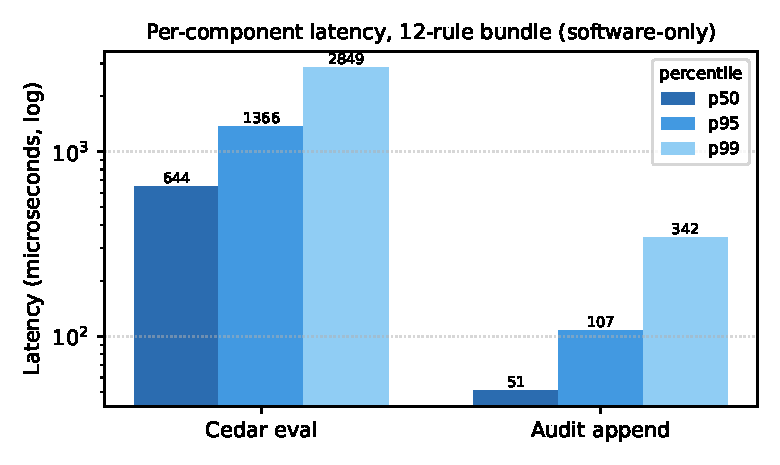
\includegraphics[width=0.78\linewidth]{figures/latency-breakdown.pdf}
\caption{Per-component latency in software-only mode against the 12-rule reference bundle
(log scale, microseconds). Cedar policy evaluation dominates; the hash-chained audit
append is roughly an order of magnitude cheaper at every percentile. Measured over 8{,}000
calls after 1{,}000 warmup calls on a single host.}
\label{fig:latency-breakdown}
\end{figure}

\begin{figure}[h]
\centering
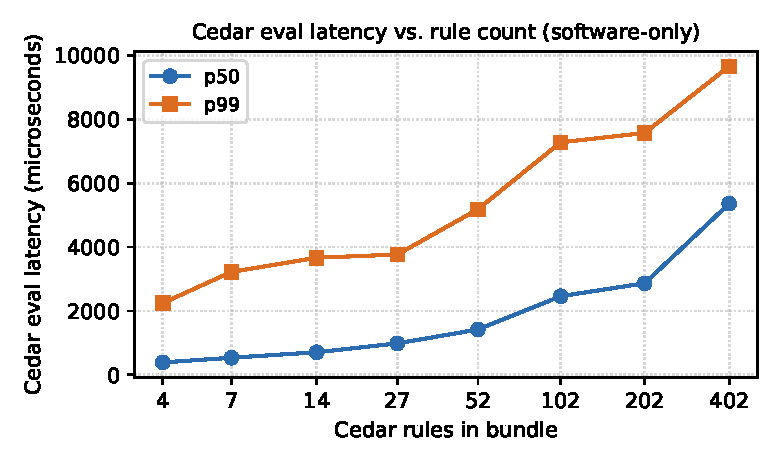
\includegraphics[width=0.78\linewidth]{figures/cedar-latency-vs-rules.pdf}
\caption{Cedar evaluation latency versus the number of rules in the policy bundle
(log-scaled x-axis, software-only mode). Median (p50) and tail (p99) latency both grow
with rule count; the underlying data appear in Table~\ref{tab:rule-scaling}.}
\label{fig:cedar-vs-rules}
\end{figure}

\begin{table}[h]
\centering
\caption{Cedar evaluation latency and single-thread throughput versus bundle rule count
(software-only, 8{,}000 measured calls per configuration). ``Rules'' counts permit plus
deny rules.}
\label{tab:rule-scaling}
\begin{tabular}{rrrrr}
\toprule
Rules & p50 (\textmu s) & p95 (\textmu s) & p99 (\textmu s) & Throughput (evals/s) \\
\midrule
4   & 384  & 936  & 2243 & 1997 \\
7   & 531  & 1227 & 3221 & 1551 \\
14  & 702  & 1686 & 3665 & 1217 \\
27  & 981  & 2125 & 3765 & 907  \\
52  & 1415 & 2800 & 5182 & 634  \\
102 & 2458 & 4780 & 7280 & 370  \\
202 & 2863 & 5634 & 7574 & 309  \\
402 & 5360 & 8043 & 9662 & 178  \\
\bottomrule
\end{tabular}
\end{table}

\subsection{Summary and CI Coverage}

Table~\ref{tab:ci-coverage} summarizes the six properties, their key metrics, and CI
test coverage.

\begin{table}[h]
\centering
\caption{Property summary and CI test coverage.}
\label{tab:ci-coverage}
\begin{tabular}{lp{4.2cm}r}
\toprule
Property & Key result & CI tests \\
\midrule
1. Policy hash binding   & 51\% avalanche; PolicyHashMismatch raised & 6 \\
2. Session sensitivity   & 2/2 violations caught; 69\% FDP          & 6 \\
3. Rug-pull detection    & 48\% avalanche; fail-closed rejection     & 6 \\
4. Key binding           & 6 sub-properties verified                 & 6 \\
5. Temporal adjacency    & 0 false negatives; denied calls recorded  & 9 \\
6. Cross-org chains      & Dual-TEE: independent verify + tamper    & 9 \\
\bottomrule
\end{tabular}
\end{table}

All six properties are covered by unit tests that run in CI on every change,
across Linux and Windows and Python 3.11, 3.12 and 3.13.

\subsection{Limitations}

\textbf{Software-only TEE.} All experiments in this paper use software-only mode. The
cMCP repository holds one hardware capture from an Azure confidential VM on AMD SEV-SNP
(July 27, 2026, \texttt{experiments/hardware-validation}): the provider verified the
VCEK certificate chain, the report signature and the nonce binding, and rejected a wrong
nonce. That capture used a fixed test nonce rather than a gateway key, and this paper does
not report hardware overhead.

\textbf{Catalog drift at the upstream server.} The measured revision pins the approved
catalog it serves but does not compare it with an upstream server's own
\texttt{tools/list}. cMCP 0.4.1 added that comparison, once per server per session; a
server that does not answer \texttt{tools/list} is recorded as unchecked and not denied.

\textbf{Security advisories.} Ten advisories were published for \texttt{cmcp-runtime}
between August 9 and September 26, 2026, all fixed by 0.6.0. Their stated affected ranges
include 0.3.0, although some concern code added after the measured revision. Those that
bear on properties in this paper: GHSA-q5qc-j6fh-5wxp (a forged TPM quote accepted as
hardware-attested, fixed in 0.4.0); GHSA-x7jr-cvph-3h7x and GHSA-h4rv-jm9x-gjf3 (a signed
SEV-SNP report and an unrelated claim accepted together, fixed in 0.5.0);
GHSA-wh6r-6j4v-p4p6 (the policy bundle hash diverges from RFC~8785 on non-ASCII and float
input, which affects the independent re-hash in Property~\ref{prop:policy-hash}(b), fixed
in 0.5.0); GHSA-xg6p-vhf6-r43q (an agent credential could reach session reset, which bears
on Property~\ref{prop:session-sensitivity}, fixed in 0.6.0); and GHSA-c8f9-q52v-fhfp (the
upstream drift check added in 0.4.1 kept its cache across a session transition, fixed in
0.6.0). Deployments should run the current release.

\textbf{FDP under agent-cooperative tagging.} The 69\% overall FDP is a worst-case figure
for the monotonic session model without agent cooperation. The runtime now accepts a per-call
\texttt{\_cmcp.data\_class} declaration and gates it on that same call. This can reduce false
positives for well-behaved agents, but it is declared sensitivity rather than independently
proven PHI lineage and therefore does not strengthen the gateway's zero-false-negative claim.

\textbf{Phase~2 simulation.} The cross-organizational attestation experiment simulates
Phase~2 in software. Real Phase~2 deployment requires a server-side TEE and an attestation
verification service, neither of which is available for evaluation in this paper.

\textbf{Synthetic traces.} FDP is measured on synthetic agent personas with hand-labeled
ground truth. Real agent behavior may exhibit different call patterns that shift the FDP
distribution.

\section{Related Work}
\label{sec:related}

\paragraph{MCP security.}
The MCP specification~\citep{mcp2024} defines the transport, the tool invocation
protocol, and OAuth-based authorization of a client to a server, but leaves per-call policy
to implementors. Concurrent work has identified
prompt-injection and tool-poisoning risks in MCP deployments~\citep{mcpsecurity2025}, where
malicious tool descriptions or responses cause an agent to take unintended actions. cMCP
addresses tool-poisoning through catalog hash pinning (Property~\ref{prop:rug-pull}) but
does not claim to prevent all prompt-injection attacks; the inspection pipeline detects
known patterns but cannot make semantic judgments about agent intent.

\paragraph{TEE-based policy enforcement.}
Using TEEs to enforce policies at runtime has been studied in the context of database
systems~\citep{teedb2017}, open enclave frameworks~\citep{keystone2020}, and network
functions~\citep{teefw2019}. The common pattern is to measure a policy into the TEE at
startup and use remote attestation to let a verifier confirm which policy was in effect.
cMCP applies this pattern to the MCP boundary, adding the dimension of session-level state
(the sensitivity state machine) that persists across multiple tool calls within a session,
rather than evaluating each request independently.

\paragraph{Agent governance frameworks.}
The Agent Governance Toolkit (AGT)~\citep{agt2026} provides the policy engine, identity
layer (SPIFFE/SVID), and Cedar policy bundle format that cMCP uses for enforcement.
cMCP acts as an enforcement point for AGT policies at the MCP boundary. Other agent
governance frameworks~\citep{guardrails2023,nemo2023} focus on output filtering and input
validation rather than tool-call interception, and do not provide hardware-backed
attestation of enforcement.

\paragraph{Attestation standards.}
RATS (Remote ATtestation procedureS)~\citep{rats2021} defines the roles and information
flows for remote attestation: Attester (the device producing evidence), Verifier (who
appraises it), and Relying Party (who makes trust decisions). TRACE~\citep{trace2025}
implements the RATS model for AI agent deployments. The TRACE Claim produced by cMCP is
an Attestation Result in RATS terminology, combining hardware evidence (the TEE
measurement report) with application-level evidence (the session call summary and audit
chain). EAT (Entity Attestation Token)~\citep{eat2023} provides the underlying token
format that TRACE extends.

\paragraph{Cryptographic audit logs.}
Hash-chained audit logs are well-studied in the context of certificate
transparency~\citep{ct2013} and secure logging~\citep{seclog2000}. The cMCP audit chain
is a linear hash chain in the style of Schneier and Kelsey: each entry commits to the hash
of its predecessor, so any deletion or modification of an entry changes the chain tip,
which is embedded in the TRACE Claim. Certificate transparency instead uses a Merkle tree,
which gives logarithmic inclusion and consistency proofs that a linear chain does not.
cMCP chains are also per-session rather than global.

\paragraph{Data provenance.}
Provenance tracking in distributed systems has a long history~\citep{prov2013}; PROV-DM
provides a data model for expressing provenance relationships. Temporal adjacency, as used
in cMCP, is a weak form of provenance: it asserts that call $B$ \emph{could} be
PHI-adjacent because it followed a PHI call, but does not assert that $B$ \emph{actually}
carries PHI-derived data. This is analogous to conservative call graph approximations in
static analysis~\citep{reps1995}, which accept false edges to achieve soundness. The
provenance disclaimer in every cMCP call graph summary (Property~\ref{prop:temporal}(c))
makes this distinction explicit.

\paragraph{Confidential computing for AI.}
Prior work applies confidential computing to machine learning~\citep{confai2024}, and
cryptographic protocols such as homomorphic encryption protect transformer inference
without trusted hardware~\citep{teeinference2023}. cMCP's use of TEEs is orthogonal: it
protects the governance layer (policy enforcement, audit) rather than the model itself.
The two approaches are composable: a model running in a TEE and a cMCP gateway both
running in TEEs can exchange mutual attestation reports, establishing end-to-end hardware
trust across the full inference-to-tool-call path.

\section{Conclusion}
\label{sec:conclusion}

cMCP is a TEE-based gateway for Model Context Protocol that provides verifiable governance
properties at the tool-call boundary. We have stated and experimentally validated six
security properties: TEE-measured policy enforcement, session sensitivity tracking, tool
catalog rug-pull detection, TRACE Claim nonce binding, temporal adjacency provenance
approximation, and cross-organizational attestation chains.

The key design decisions and their consequences are:

\textbf{Hardware binding over software assertion.} The nonce construction ties each TRACE
Claim to a specific TEE startup instance and session. A claim presented as evidence cannot
be replayed from a different instance or session without breaking the Ed25519 signature or
the nonce-report\_data binding.

\textbf{Monotonic session state over per-call evaluation.} The session sensitivity state
machine catches cross-boundary PHI violations that per-call policy evaluation structurally
cannot. The cost is a quantified false-discovery proportion (69\% overall in our evaluation) that
motivates Phase~2 agent-cooperative tagging.

\textbf{Fail-closed catalog pinning over advisory warnings.} A catalog that differs from
its approved hash stops the gateway at load time, and a change to the in-memory catalog
after startup stops the call. This prevents rug-pull attacks at the cost of requiring catalog updates to go through
a re-attestation cycle.

\textbf{Open problems.} Three problems are left open. First, Phase~2 server TEE deployment
is in progress; the dual-TEE cross-organizational protocol has been simulated but not
demonstrated with physical hardware. Second, the runtime now accepts a per-call \texttt{\_cmcp.data\_class}
declaration, but that is declared sensitivity; an SDK-level convention for agents to prove
PHI lineage does not yet exist.
Third, semantic attacks, where a compliant-looking tool response causes harmful agent
behavior, are outside the scope of the current inspection pipeline.

The cMCP implementation and all experiments are available at
\url{https://github.com/agentrust-io/cmcp} under the MIT license.


\bibliographystyle{plainnat}
\bibliography{refs}

\end{document}
